\documentclass{beamer}
\usepackage{beamerthemeshadow}
%\usepackage{natbib}
\usepackage{amssymb,amsmath,amsthm,mathrsfs,mathtools,amscd,stmaryrd}
\usepackage{mathrsfs}
\beamersetuncovermixins{\opaqueness<1>{25}}{\opaqueness<2->{15}}
%\usetheme{Pittsburgh}
\usepackage{listings}
\usepackage{color}

%\synctex=1

\useinnertheme{rounded}
\usecolortheme{fly}
\setbeamercolor{normal text}{bg=white!20} 
\setbeamercolor{title}{bg=brown!20!gray}
\setbeamercolor{block title}{fg=black,bg=brown!10!gray!30!}
%\setbeamercolor{frametitle}{fg=dw-blau,bg=dw-blau!10}
\setbeamercolor{section in head/foot}{fg=white,bg=brown!20!gray!80!}
\setbeamercolor{author in head/foot}{fg=white,bg=brown!20!gray!70!}
\setbeamercolor{title in head/foot}{fg=white,bg=brown!20!gray!60!}
\setbeamercolor{subsection in head/foot}{fg=white,bg=brown!20!gray!}%

\setbeamercolor{section in toc}{fg=black}
%\logo{\includegraphics[height=0.4cm]{Drocon_Label.pdf}} 
\setbeamercolor{logo}{bg=white}
\setbeamercolor{itemize item}{fg=gray}
\setbeamercolor{itemize subitem}{fg=blue!30!gray!80!}
\newenvironment{recap}{\begin{small}\color{gray}\begin{flushright}}{\end{flushright}\end{small}}


\begin{document}

\title{Correct and Efficient Citation Management with Jabref}

\author[J. Heiland ]{Jan Heiland}

\institute{Tool Seminar, AG Mehrmann}
\date{January 12, 2012} 
\titlegraphic{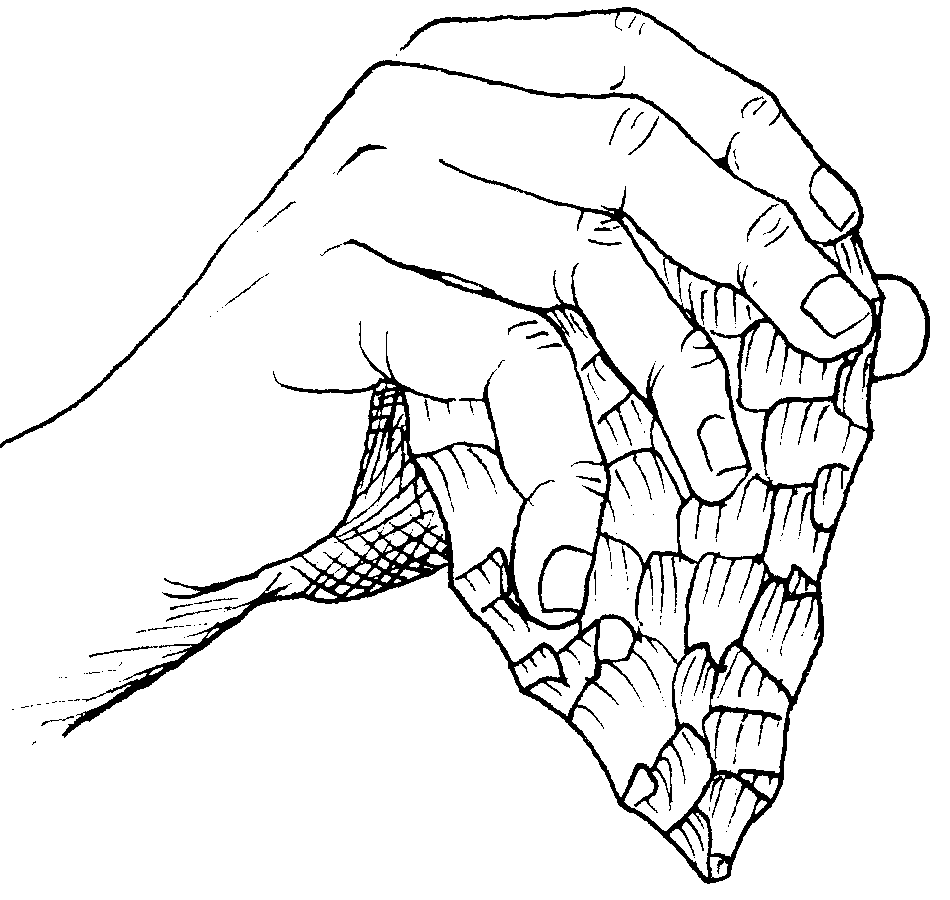
\includegraphics[scale=0.081]{Agarre_de_un_bifaz.png}}
\frame{\titlepage} 


\frame{
%\frametitle{Content/Purpose}
\tableofcontents
}
\section{Latex, Bibtex and bib-files}
\begin{frame}[fragile]
How bibtex is used 
\definecolor{darkgreen}{rgb}{0,0.6,0}
\begin{small}
	\lstset{language=[LaTeX]TeX,
texcsstyle=*\bf\color{blue},
numbers=none,
breaklines=true,
keywordstyle=\color{darkgreen},
commentstyle=\color{darkgreen},
frame=none,
tabsize=2}
	\begin{lstlisting}


		\documentclass{article}
		\usepackage{cite}	% package for the use of BibTex

		\begin{document}

		blabla, cf. \cite{Bec05} % cite a reference

		\bibliography{toolSem1} % use bib-file toolSem1.bib
		\bibliographystyle{plain}

		\end{document}
	\end{lstlisting}
\end{small}
\ldots see our webpage for this example and further reading \ldots
\end{frame}

\begin{frame}[fragile]
A bibtex file\ldots

	\ldots a bib file is a plain text file that contains arbitrary high numbers of bib-entries

	\begin{small}
		\begin{lstlisting}

			@BOOK{Cia02,
			title = {The finite element method for elliptic problems},
			publisher = {SIAM},
			year = {2002},
			author = {Ciarlet, P. G.},
			volume = {40},
			series = {Classics in Applied Mathematics},
			address = {Philadelphia, PA}
			}

		\end{lstlisting}
	\end{small}

	and Jabref can help to handle it\ldots
	
\end{frame}

\section{Handling of bib-files with Jabref}
\subsection{Jabref}

\frame{
Jabref \ldots
\begin{itemize}
	\item \ldots is GPL software 
	\item \ldots comes for all platforms
	\item \texttt{http://sourceforge.net/projects/jabref/}
\end{itemize}
}
\subsection{Basic Functionality}

\frame{
Jabref can
\begin{itemize}
	\item open several bibs in a GUI
	\item sort them by author, title, year, etc.
	\item copy and paste between the libs
	\item edit the entries
	\item assign files like PDFs to the entries
\end{itemize}
\vfill
\hfill
$\rightarrow$ watch the live performance
}
\subsection{Import of Bib-Entries}

\frame{
Importing of bibtex entries 
\begin{itemize}
	\item via copy-n-paste from other bib-files
	\item from plain text
	\item from the internet [later]
\end{itemize}
\vfill
\hfill
$\rightarrow$ watch the live performance 
}

\subsection{Interplay with the Latex Editor}

\frame{
ctrl-K copies  ``$\backslash$cite$\{$currentKey$\}$`` to the clipboard
\vfill
\hfill
$\rightarrow$ watch the live performance
}

\section{Citations in Math-Manuscripts}
\subsection{Where to Take from}

\frame{
Bibtex entries are provided by most of the services that list or host scientific papers. In particular for mathematics it may be worth checking
\begin{itemize}
	\item \texttt{http://www.ams.org/mathscinet/index.html}
	\item \texttt{http://www.zentralblatt-math.org/zmath/en/search/} ( features a ``TU'' button )
	\item \texttt{http://www.sciencedirect.com/}
	\item \texttt{\ldots}
\end{itemize}
and also most of the preprint servers\ldots

}
\subsection{When to Use}

\frame{
???

\vfill
are there any rules or best practices\ldots
\vfill

For an overview of phrases and formulations see the book by Treziak: \textit{Writing Mathematical Papers in English}
}

\end{document}
